\chapter{Architectural Design}
\section{Overview: high-level components and interactions}

As anticipated in the previous chapter, the architecture selected for the design and development of the system is the three-tier architecture.

This architecture allow us to split the implementation into three layers:
\begin{enumerate}
	\item Presentation: is the mobile application that will be used by the final users. It allows all the interactions with the system and will also be used as a communication endpoint for the notifications.
	\item Application: is the backend of the system, all the business logic and the various connections between the system and the external services are implemented here.
	\item Data: is the layer responsible to expose connectivity interfaces from the database. It will be a DBMS.
\end{enumerate}
All the layers communicate in a linear way: the Presentation one interacts only with the Application layer, the same as the Data layer. With this architecture the presentation and the Data layers have no direct communication path, this allow to develop all the business logic only in the Application layer.
Other advantages of using this architecture are that the various layers can be developed with different technologies and that they can be duplicated and differentiated (i.e. there can be multiple presentation layers that interact with the same application layer)

The main reasons behind the choice are:
\begin{itemize}
	\item We are not the producer of the data
	\item We need to integrate different external services
	\item Separate the business logic from the data to:
	\begin{itemize}
		\item Allow a parallel development with multiple teams specialized in the single tiers
		\item Allow to use different technologies for the different tiers
	\end{itemize}
\end{itemize}


\begin{figure}[h]
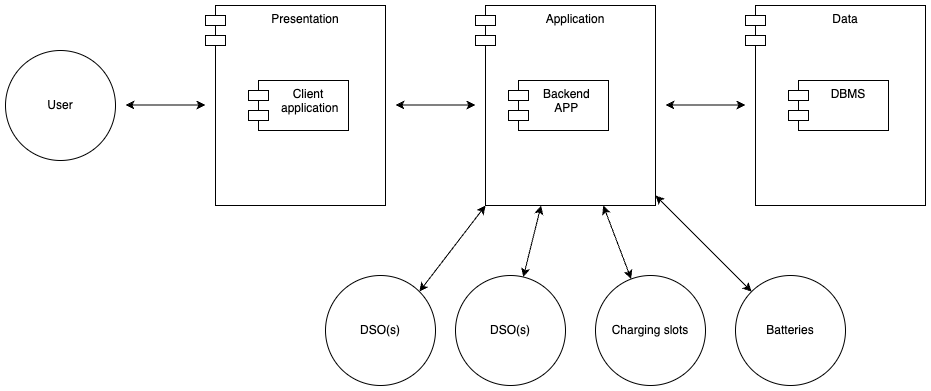
\includegraphics[width=\textwidth]{component_diagrams/overview}
\caption{Overview of the chosen three-tier architecture with actors}
\end{figure}

\clearpage

\section{Component view}
The following schema shows all the main components and interfaces of the system. Later on you will find the details of each component.


\begin{figure}[h]
\centering
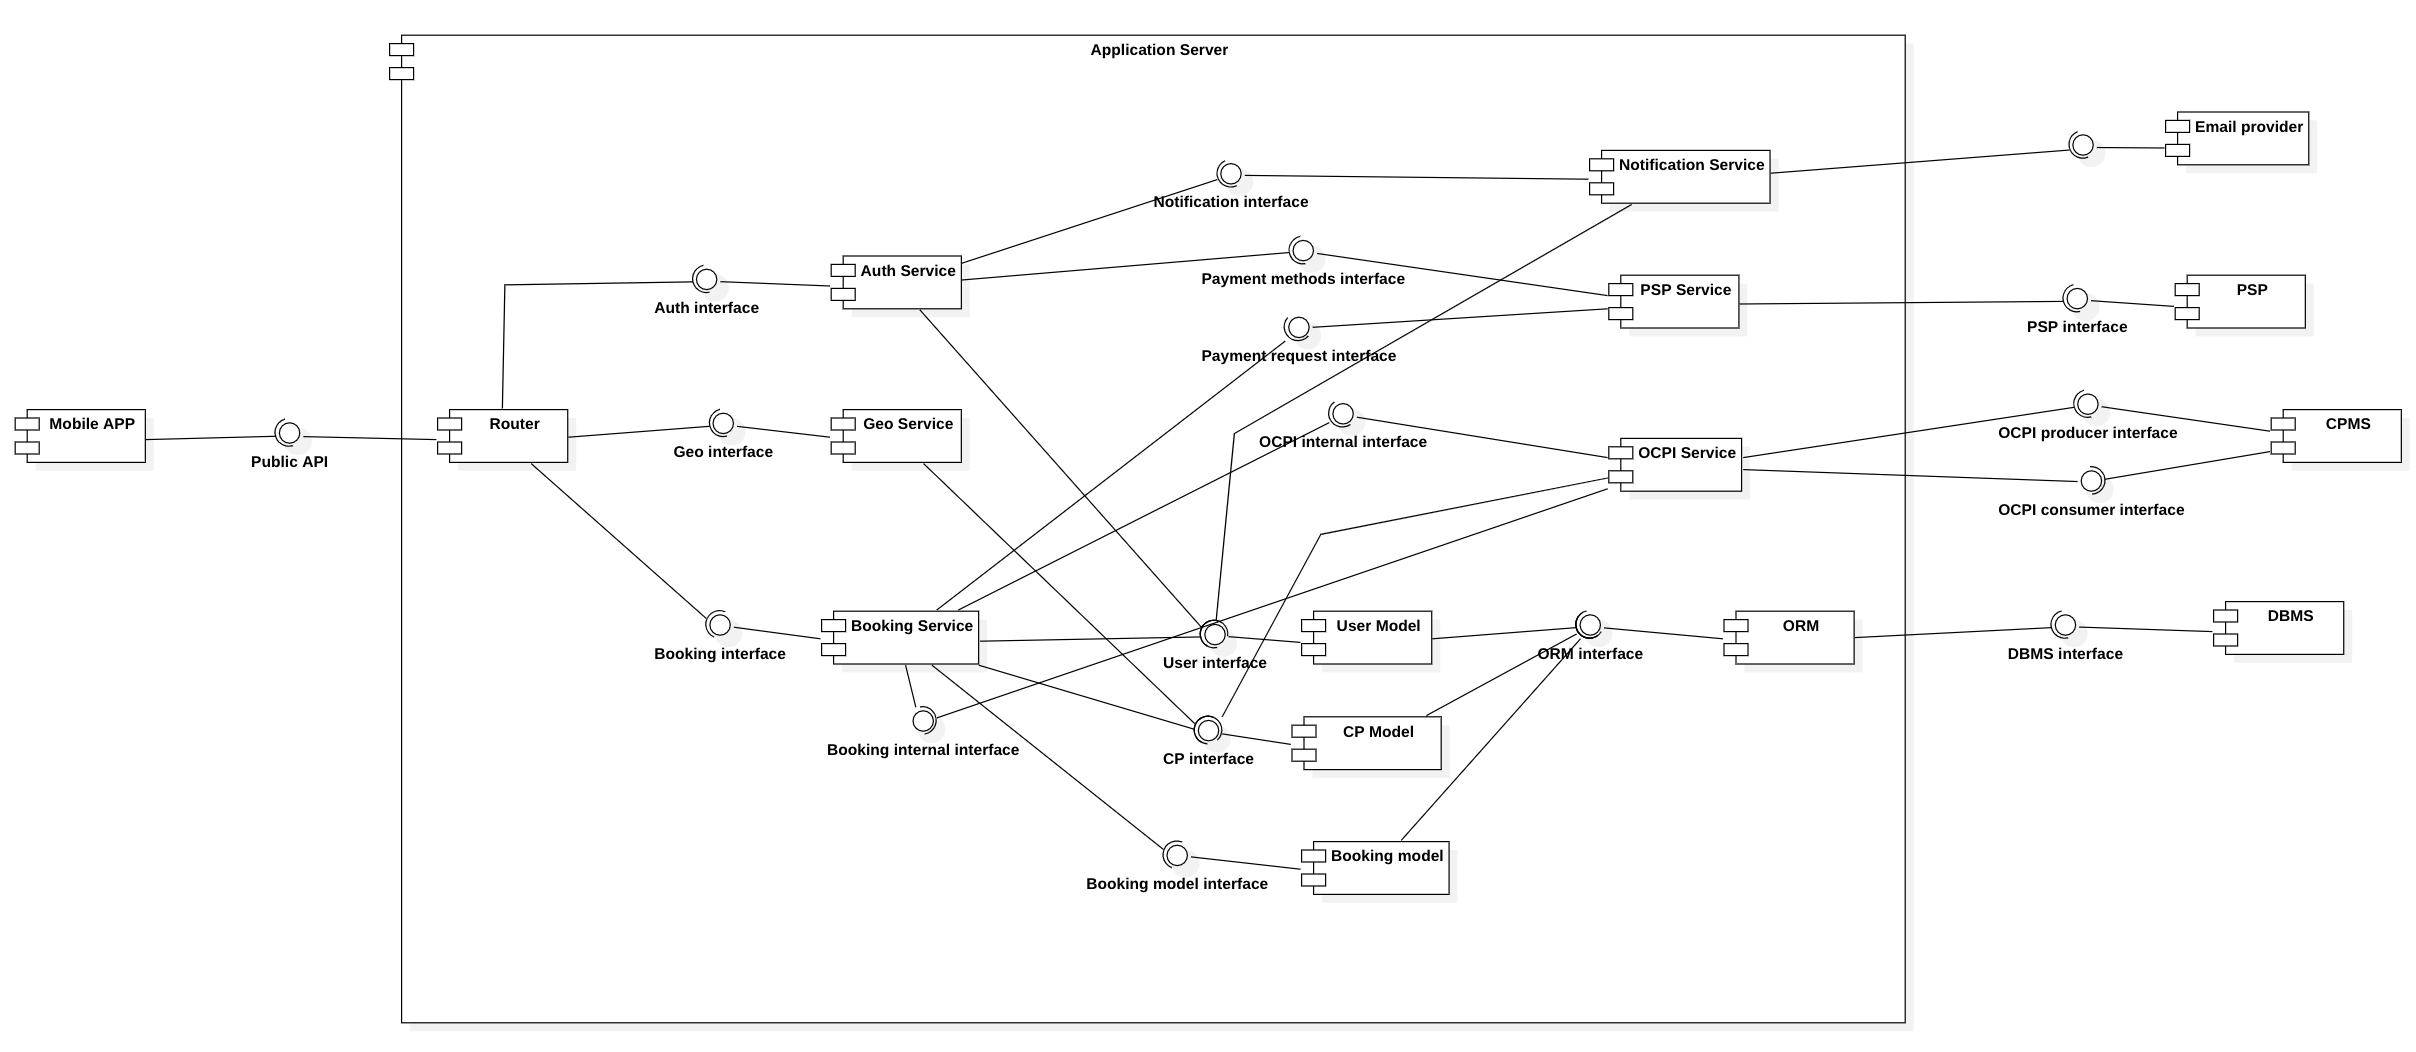
\includegraphics[angle=90,origin=c,height=14cm]{component_diagrams/component_diagram}
\caption{Component diagram of the system}
\end{figure}

\clearpage
\newpage

\begin{itemize}
	\item \textbf{Application server}: not a real "component" it shows the division between the backend, the frontend, the data layer and the external service. In the three-tier architecture it represents the Application layer.
	\item \textbf{Mobile APP}: mobile application for the system, used by the users.
	\item \textbf{Router}: handles all the requests directed to the Application APIs (i.e. OCPI PUSH endpoints are not handled here) that comes into the Application Server, uses the Auth Service to Authenticate and Authorize them. After that, if all the checks are passed, it will forward the request to the correct service that exposes the required route. It basically acts as a middleware, its presence is useful as it acts as a single point to develop all the authentication/authorization logic so that if it needs changes we can just update the router (and eventually the auth service) instead of updating all the services.
	\item \textbf{Auth Service}: is an internal service that handles authentication (Signup and login) and authorization (even if at the moment our system does not need that). It is mainly used internally but it exposes a couple of endpoints to the router for both signup and login.
	\item \textbf{Geo Service}: an highly reusable service, it uses a set of geographical points and exposes functionalities to list, filter and search those points based on their position. For our system is needed for the map functionality of the Mobile APP.
	\item \textbf{Booking Service}: it manages the booking for the application, it exposes some endpoints to the router for the booking functionalities of the Mobile APP and it is also used from other internal services.
	\item \textbf{Notification Service}: it manages all the notifications that the system needs to send to the user, both via email as via push services (e.g. Firebase Cloud Messaging)
	\item \textbf{PSP Service}: it manages the communication with the Payment Service Providers, it is useful as we can easily swap it with proprietary SDKs from the various providers.
	\item \textbf{OCPI Service}: it manages the communication with the CPMS, it exposes the endpoints for the PUSH part of the protocol (is needed to receive real-time updated from CPMS)
	\item \textbf{ORM}: a library that allows an easy to use mapping between Models and DB table, it handles queries and relationships. It is not worth it to develop an in-house solution, so we will use a library for that.
	\item \textbf{User Model, CP Model, Booking Model}: Models components that sit between services and ORM, useful to attach event listeners and other effects that need to run when updating the data. 
	\item \textbf{Email Provider}: external service (or services) that exposes API to send emails
	\item \textbf{PSP}: external service that exposes API to process payment
	\item \textbf{CPMS}: Charging Point Management System that exposes OCPI compliant API
	\item \textbf{DBMS}: Database Management System
\end{itemize}

\clearpage
\subsection{Class diagram}
\begin{figure}[h]
\includegraphics[width=\textwidth]{class_diagram}
\caption{Class diagram for the main models of the System}
\end{figure}
\clearpage
\newpage

\section{Deployment view}
In this section we introduce a detailed view of the system and various component from a deployment cycle perspective. The following schemes highlight the environments and the tools to be used for the system.
\begin{figure}[h]
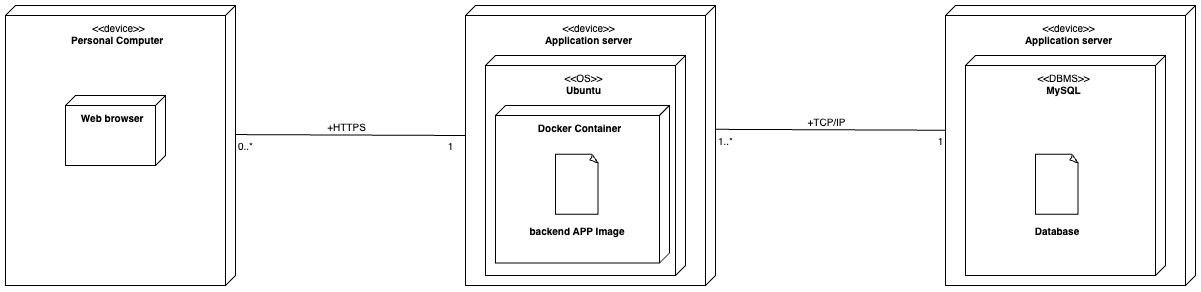
\includegraphics[width=\textwidth]{component_diagrams/deployment_diagram}
\caption{Deployment diagram for the System}
\end{figure}

\begin{itemize}
	\item \textbf{Personal Device}: Mobile device used by users to run the Mobile APP to communicate with the system
	\item \textbf{Load Balancer}: A web server that balances incoming requests between multiple backend servers
	\item \textbf{Backend Server / Virtual Private Server}: Physical device where is installed the Docker Image of the Backend APP. Multiple replicas are possibile and preferable as they will increase both reliability and availability of the system. Keep in mind that without replicating the data layer, there will always be a bottleneck of performances due to the communication between application and data layers.
	\item \textbf{Database Server}: Host the database of the system. Multiple local replicas can improve read performances but also increase complexity.
\end{itemize}

\clearpage
\newpage

\section{Component interfaces}
In this section we introduce the main interfaces of the various components of System. 
\begin{figure}[h]
\includegraphics[width=\textwidth]{component_diagrams/class_diagram}
\caption{Component interfaces diagrams for the system}
\end{figure}

\clearpage
\newpage


\section{Runtime view}
In this section are shown the sequence diagrams for the various functionalities of the system. To simplify the description there is an initial generic sequence the summarize the routing and authorization part of the request handling. Also, as all the request go through the router, the actors that sends the request to the router are omitted.

\subsection{Generic Routing and Authorization}
\begin{figure}[h]
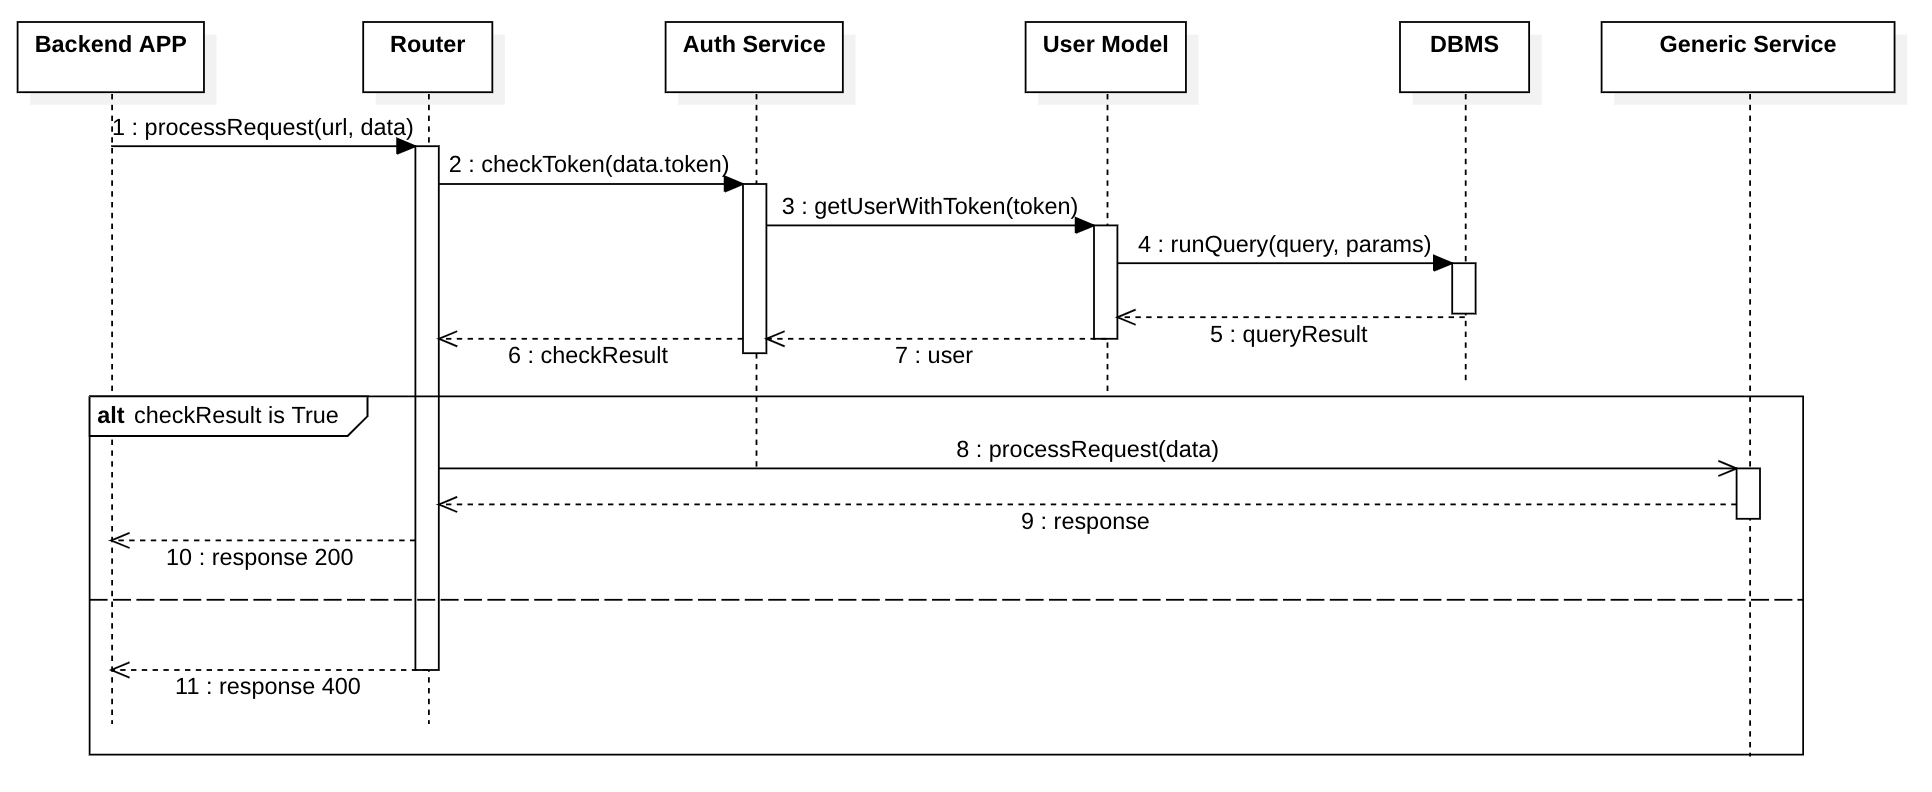
\includegraphics[width=\textwidth]{sequences/auth_request}
\caption{Generic Routing and Authorization flow for a generic request}
\end{figure}

When a request is received by the application web server, it goes through the Router component. It acts as an authorization middleware. 
As Authorization is needed, the whole Auth Service, Model and DBMS components are envolved.
At the end, if authorization has been completed successfully, the request is forward to the dedicated service.


\subsection{View Charging Point locations}
\begin{figure}[h]
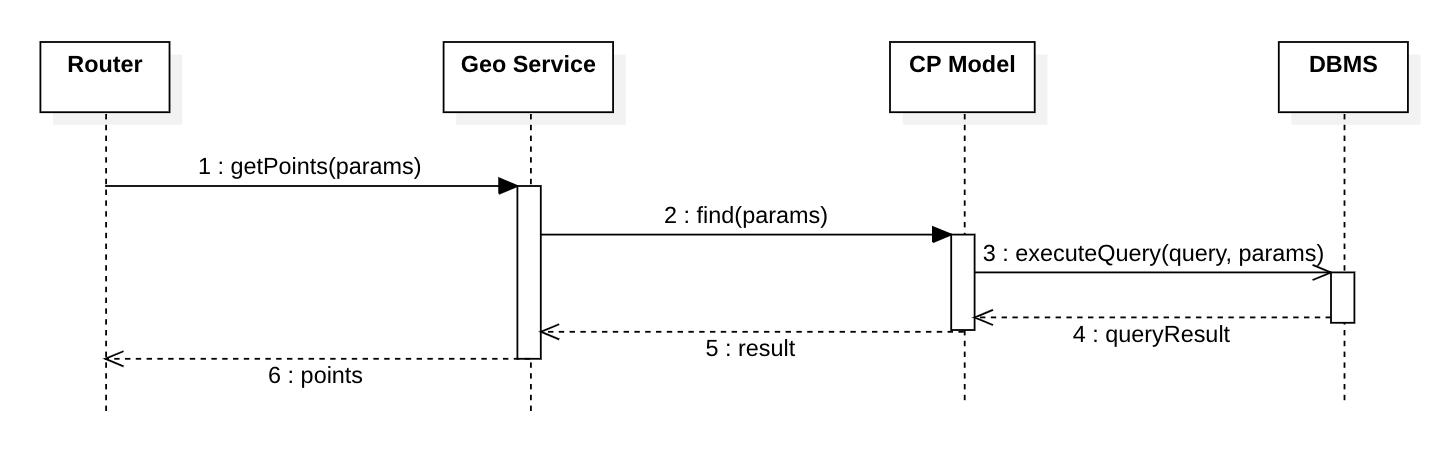
\includegraphics[width=\textwidth]{sequences/get_locations}
\caption{View Charging Point locations}
\end{figure}
\clearpage

\subsection{Book a charging session}
\begin{figure}[h]
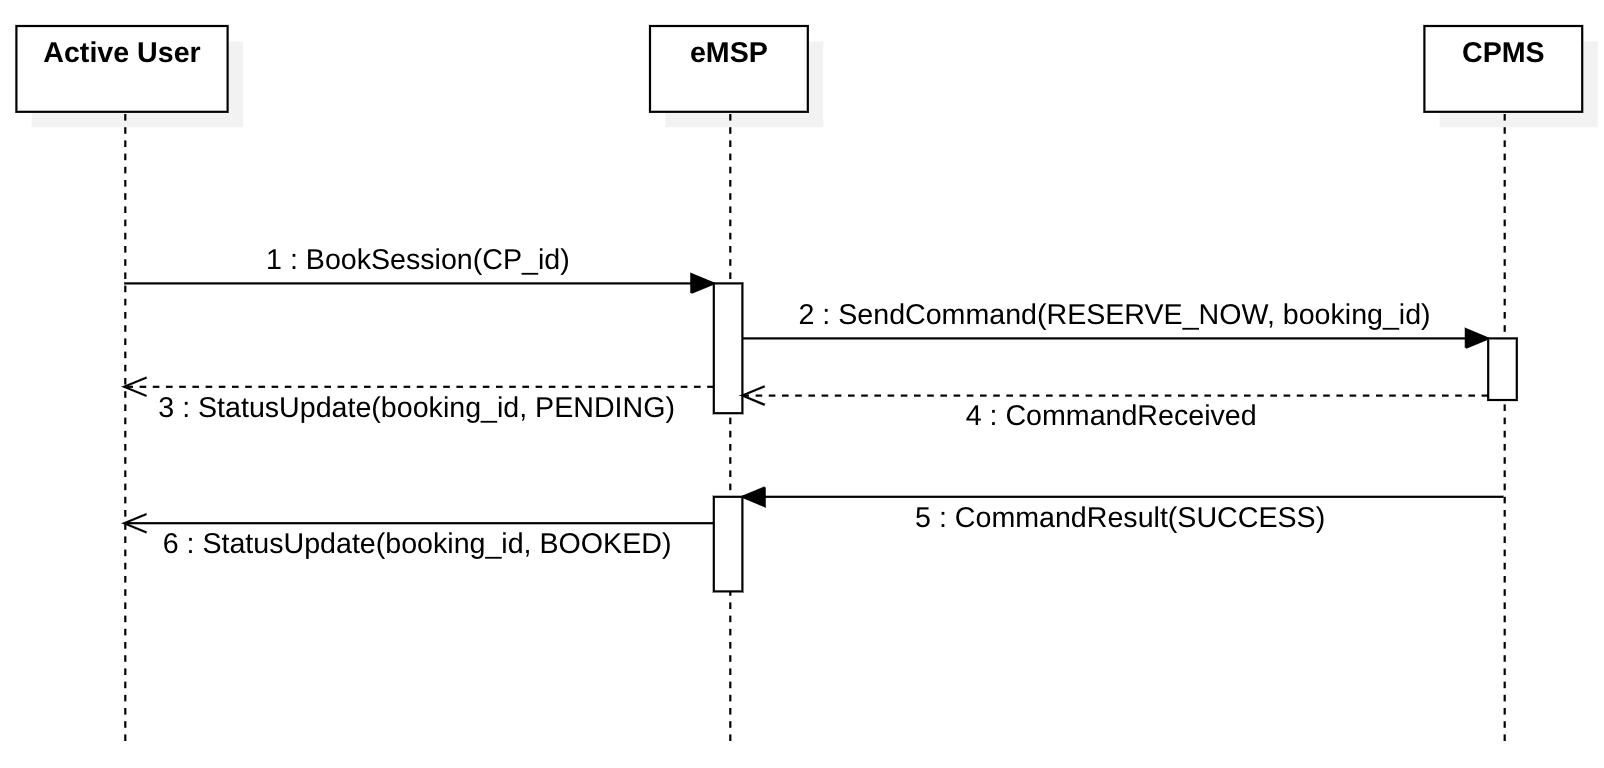
\includegraphics[width=\textwidth]{sequences/book_session}
\caption{Book a charging session}
\end{figure}

\subsection{Start a charging session}
\begin{figure}[h]
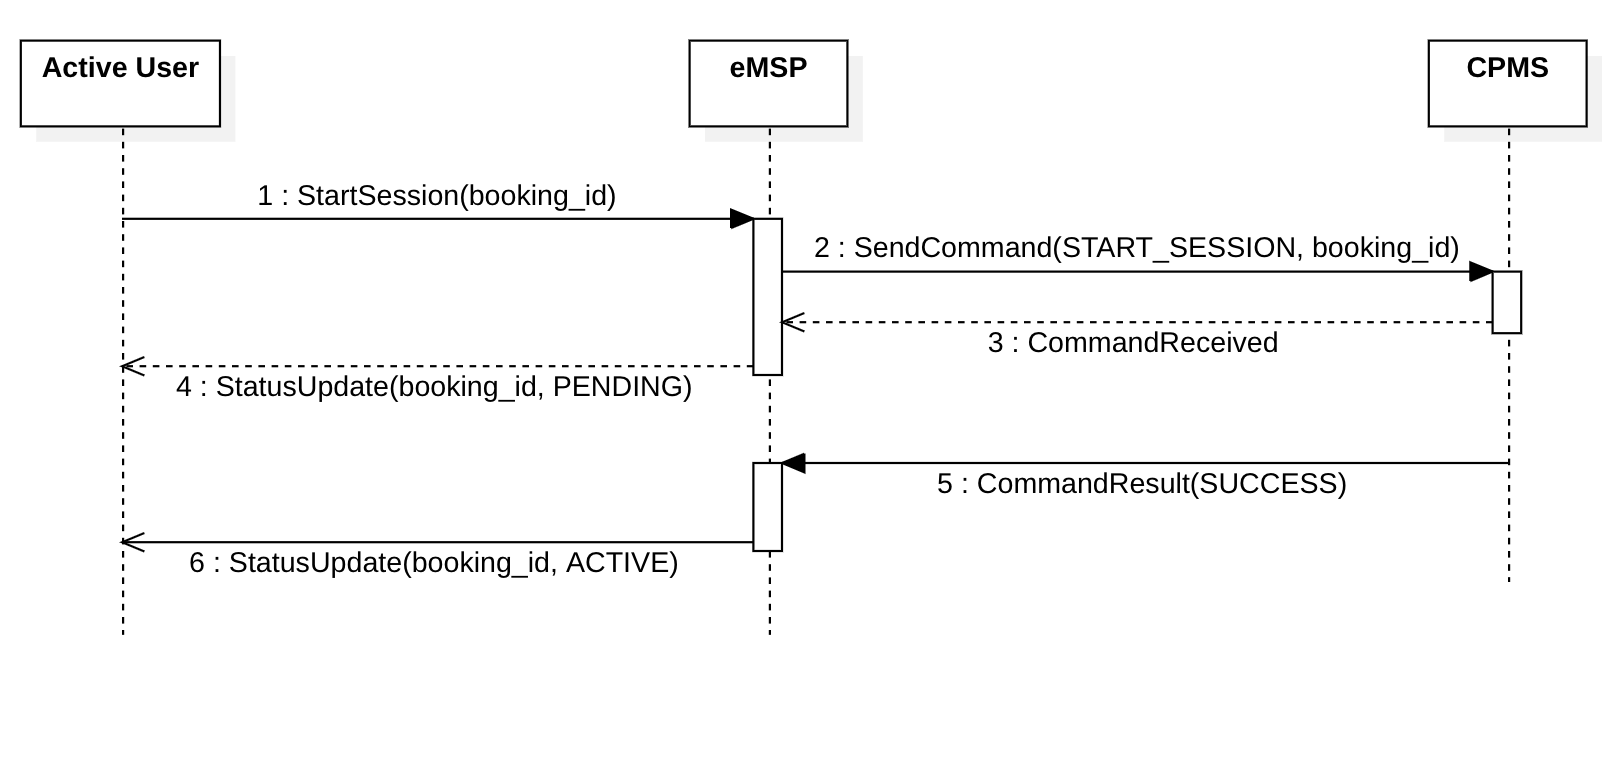
\includegraphics[width=\textwidth]{sequences/start_session}
\caption{Start a charging session}
\end{figure}
\clearpage

\subsection{Pay for a completed charging session}
\begin{figure}[h]
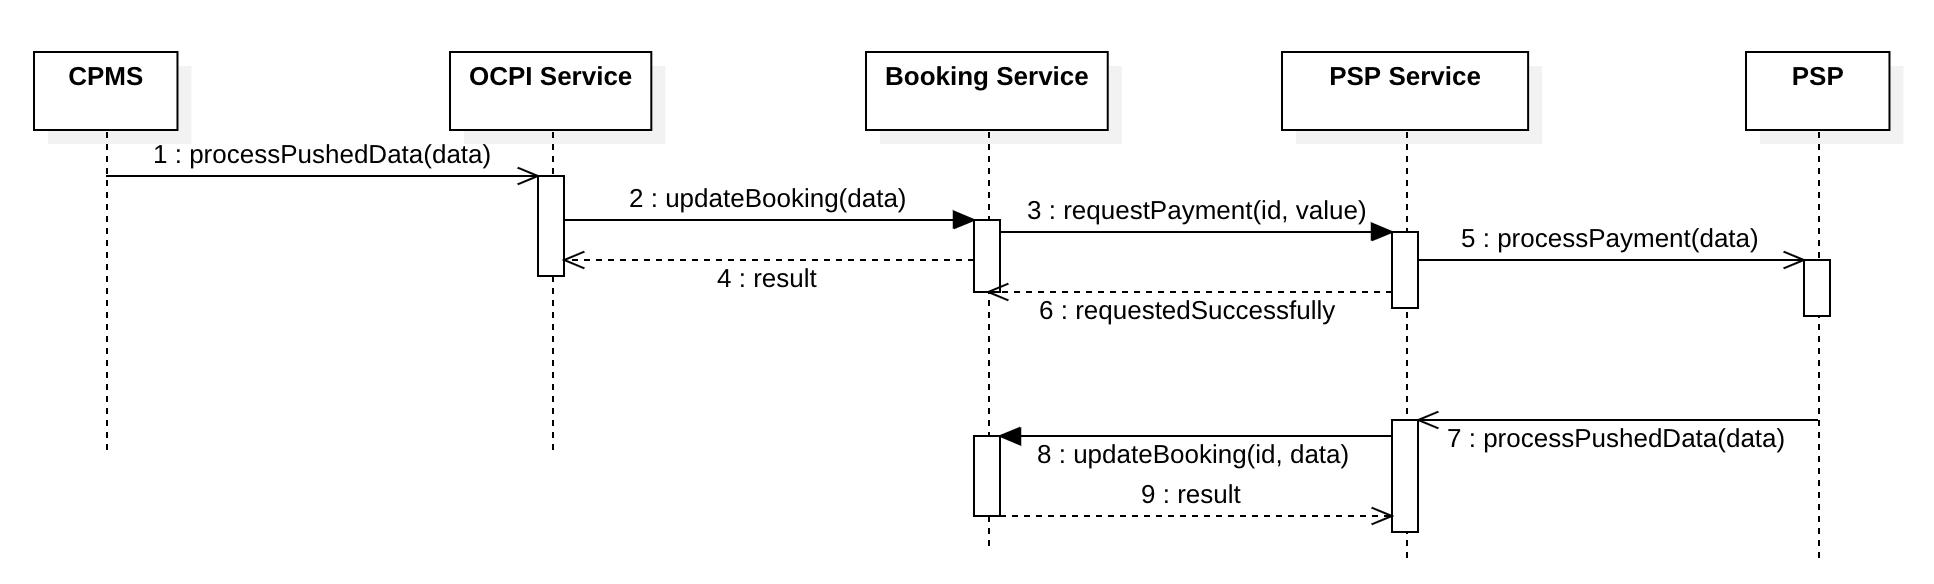
\includegraphics[width=\textwidth]{sequences/session_payment}
\caption{Pay for a completed charging session}
\end{figure}
\clearpage

\section{Selected architectural style and patterns}
\begin{itemize}
	\item \textbf{Three-tier architecture}: As stated before the three-tier architecture was chosen because our system is not the producer of the data, and that there is the need for implementing different functionalities (e.g. payments) and external services.
	\item \textbf{Monolith architecture}: To simplify the development and the deployment of the system, to avoid the so called "vendor lock-in" by choosing a specific service provider for the microservices infrastructure and mainly because no usage spikes are expected, the monolith architecture has been chosen. That means that all the application server replicas contains the whole backend application and not the single services.
	\item \textbf{Authentication with Access Token}: As there are no specific requirements on the authentication functionality, the simply access token pattern can be considered a good suit for the system. 
\end{itemize}











